\begin{figure}[h!]
    \centering
    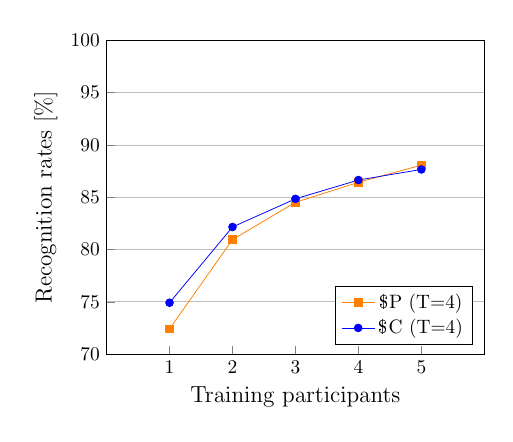
\begin{tikzpicture}[scale=.7]
        \begin{axis}[
            xlabel={\large{Training participants}},
            ylabel={\large{Recognition rates [\%]}},
            xmin=0, xmax=6,
            ymin=70, ymax=100,
            xtick pos=bottom,
            ytick pos=left,
            xtick={1,2,3,4,5},
            ytick={70,75,80,85,90,95,100},
            legend pos=south east,
            ymajorgrids=true
        ]
            \addplot[color=orange,mark=square*]
                coordinates {(1, 72.42) (2, 80.95) (3, 84.52) (4, 86.43) (5, 88.07)};
            \addplot[color=blue,mark=*]
                coordinates {(1, 74.92) (2, 82.16) (3, 84.85) (4, 86.65) (5, 87.66)};
            \legend{\$P (T=4), \$C (T=4)}
        \end{axis}
    \end{tikzpicture}%
    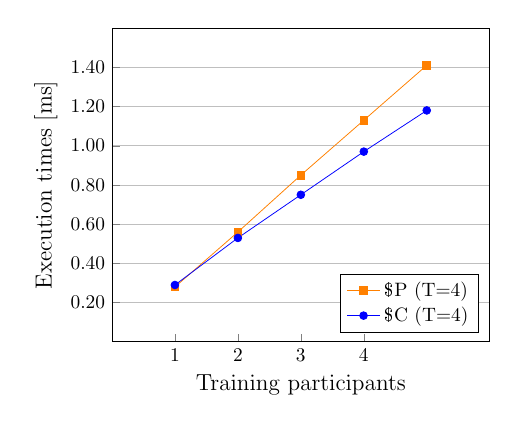
\begin{tikzpicture}[scale=.7]
        \begin{axis}[
            xlabel={\large{Training participants}},
            ylabel={\large{Execution times [ms]}},
            xmin=0, xmax=6,
            ymin=0, ymax=1.6,
            xtick pos=bottom,
            ytick pos=left,
            xtick={1,2,3,4},
            ytick={0.2,0.4,0.6,0.8,1,1.2,1.4},
            legend pos=south east,
            ymajorgrids=true,
            y tick label style={
                /pgf/number format/.cd,fixed,fixed zerofill,precision=2,/tikz/.cd
            }
        ]
            \addplot[color=orange,mark=square*]
                coordinates {(1, 0.28) (2, 0.56) (3, 0.85) (4, 1.13) (5, 1.41)};
            \addplot[color=blue,mark=*]
                coordinates {(1, 0.29) (2, 0.53) (3, 0.75) (4, 0.97) (5, 1.18)};
            \legend{\$P (T=4), \$C (T=4)}
        \end{axis}
    \end{tikzpicture}
    \caption{User-independent platform-independent testing of \$P and \$C in terms of recognition rates [\%] and execution times [ms], when the recognizers are trained with gestures performed on a tablet and tested with gestures performed on a smartphone.}
    \label{fig:cdollar_ui_pi_t}
\end{figure}